\documentclass[../AnalysisNoteJBuxton.tex]{subfiles}
\begin{document}

\subsection{Results: \texorpdfstring{$\Lambda$K$^{0}_{S}$ and $\Lambda$K$^{\pm}$}{TEXT}}
\label{ResultsLamK}

In the following sections, we present results assuming (i) no residual correlations (Sec. \ref{ResultsLamK_NoRes}), (ii) three residual contributors (Sec. \ref{ResultsLamK_3Res}), and (iii) ten residual contributors (Sec. \ref{ResultsLamK_10Res}).  We find the case of three and ten contributors to be consistent, therefore we will quote the result utilizing three residuals as our final result.  The results shown, unless otherwise noted, use a polynomial fit to the THERMINATOR simulation to handle the non-flat background, and \LamKchPALamKchM radii are shared with \LamKchMALamKchP.


I first collect all of the summary results, and will show the actual fits to the data in Sections \ref{ResultsLamK_NoRes}, \ref{ResultsLamK_3Res}, and \ref{ResultsLamK_10Res}.  In the first of the summary plots, we show the extracted scattering parameters in the form of a Im[f$_{0}$] vs Re[f$_{0}$] plot, which includes the d$_{0}$ values to the right side.  The next three summary plots show the $\lambda$ vs. Radius parameters.  The first group of plots shows: 1) results without any residual correlations included in the fit (marked as "QM 2017"), 2) results with 10 residual pairs included, and 3) results with 3 residual pairs included.  The second group of plots also includes the case where we fixed the d$_{0}$ parameter to zero.

%%%%%%%%%%%%%%%%%%%%%%%%%%%%%%%%%%%%%%%%%%%%%%%%%%%%%%%%%%%%%%%%%%%%%%%%%%%%%%%%%%%%%%%%%%%%%%%
\begin{comment}

\begin{figure}[h]
  \centering
  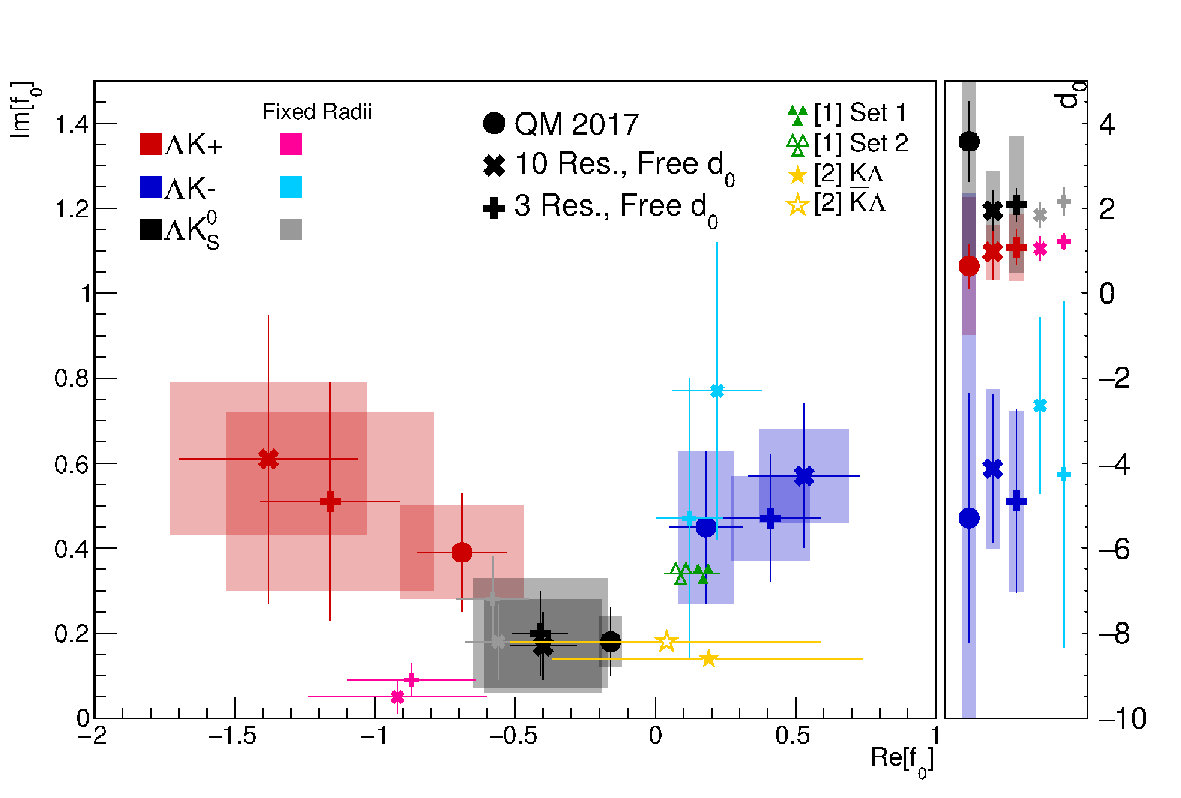
\includegraphics[width=\textwidth]{7_ResultsAndDiscussion/Figures/CompareAllReF0vsImF0AcrossAnalyses_10ResAnd3Res_10and3SeparateOnly_FreeD0Only_wFixedRadiiResults_wScattLenPredictions.pdf}
  \caption[Scattering Parameter Results]{Extracted scattering parameter results, Im[f$_{0}$] vs. Re[f$_{0}$], together with d$_{0}$ to the right, for all of our $\Lambda$K systems.  The plot shows results including no residuals (circles), 10 residual pairs (X), and 3 residual pairs (+).  The lighter color markers (pink, sky blue, gray) show the extracted parameters when we fix the radii to roughly align with the $m_{\mathrm{T}}$-scaling plot, Fig. \ref{fig:mTScalingOfRadii_NoRes}.  The green \cite{Liu:2006xja} and yellow \cite{Mai:2009ce} points show theoretical predictions made using chiral perturbation theory.  Note, \LamKchP on the plot is shorthand for \LamKchP and \ALamKchM, and similar for the others.}
  \label{fig:ImF0vsReF0_FreeD0Only}
\end{figure}


\begin{figure}[h]
  \centering
  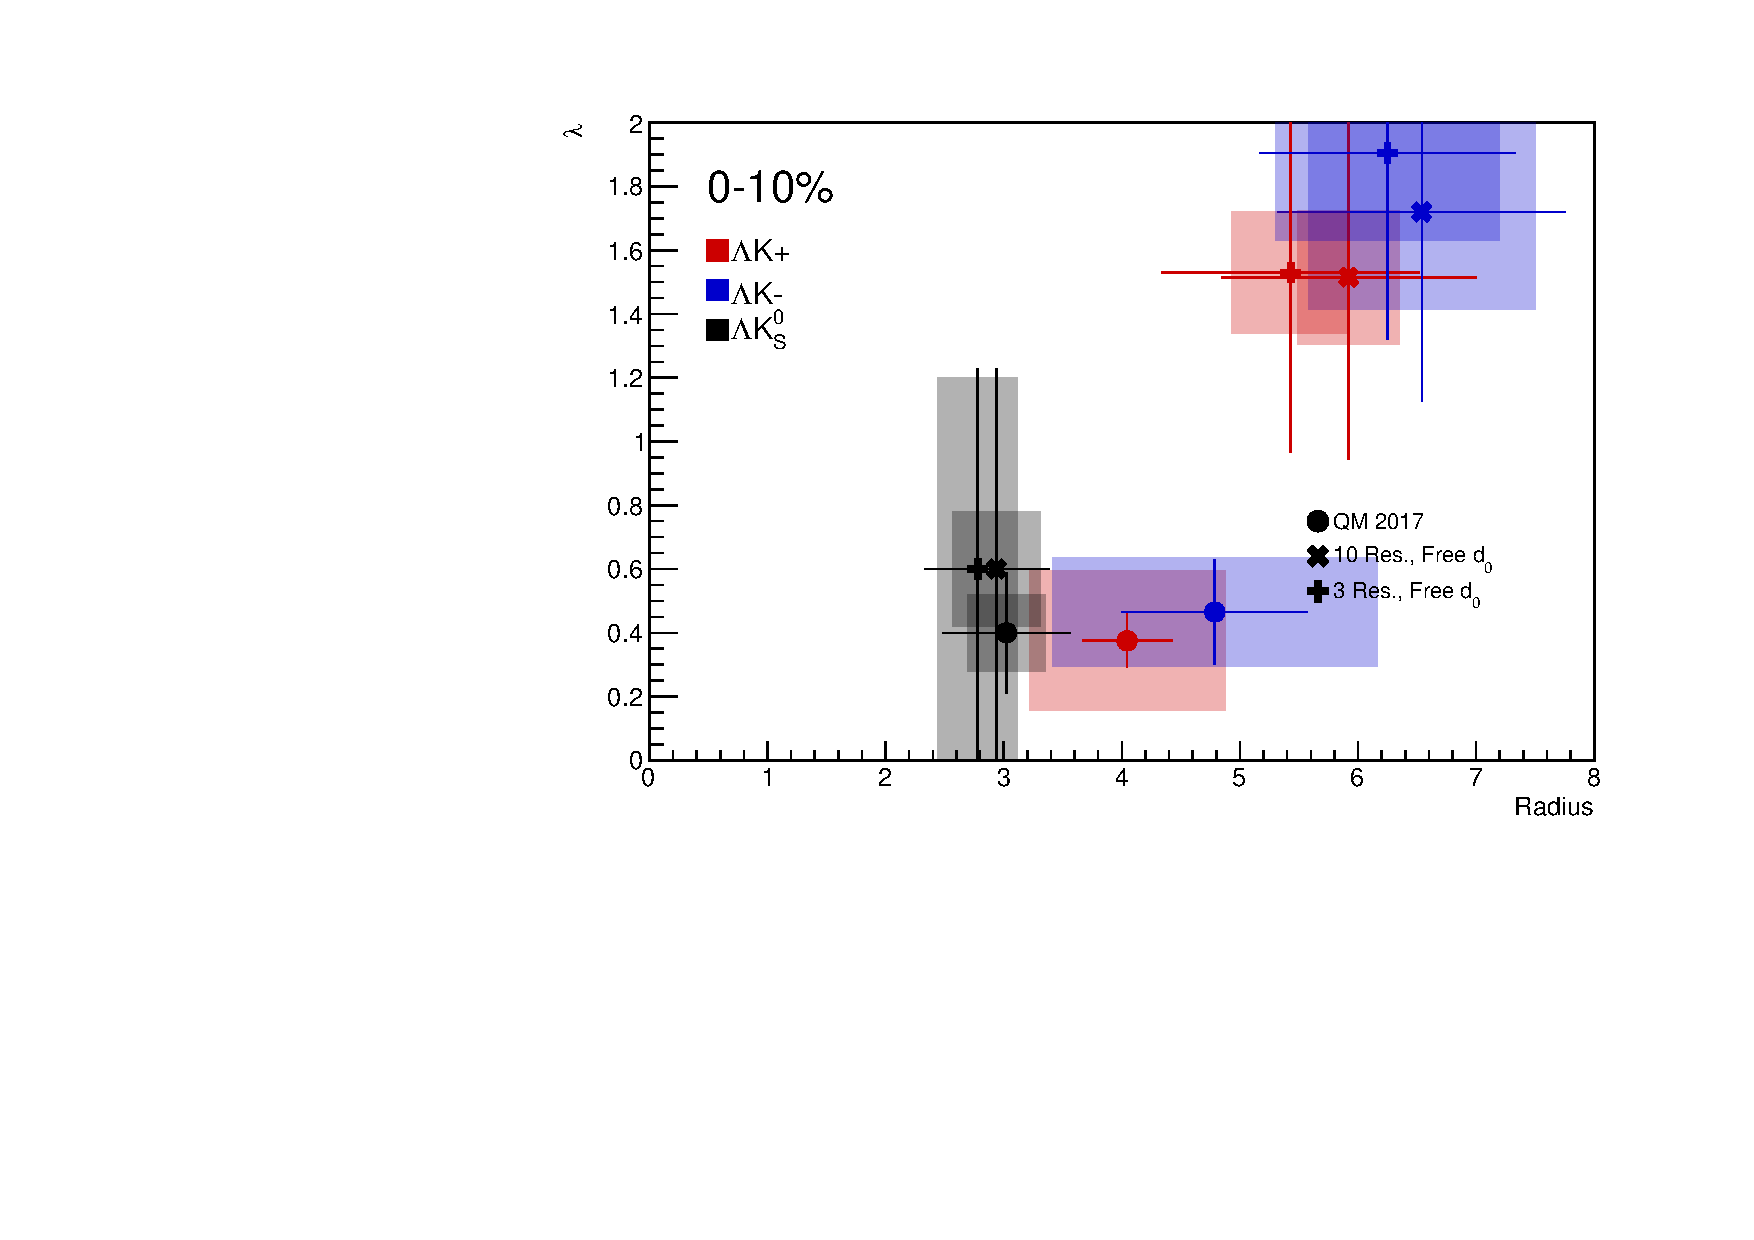
\includegraphics[width=\textwidth]{7_ResultsAndDiscussion/Figures/CompareAllRadiusvsLambdaAcrossAnalyses_0010_10ResAnd3Res_10and3SeparateOnly_FreeD0Only.pdf}
  \caption[$\lambda$ vs. R (0-10\% Centrality)]{Extracted $\lambda$ vs Radius results, for the 0-10\% centrality bin, for all of our \LamKchP systems.  The plot shows results including no residuals (circles), 10 residual pairs (X), and 3 residual pairs (+).  Note, $\Lambda$K$^{+}$ on the plot is shorthand for $\Lambda$K$^{+}$ and $\bar{\Lambda}$K$^{-}$, and similar for the others.}
  \label{fig:LambdavsR_0010_FreeD0Only}
\end{figure}

\begin{figure}[h]
  \centering
  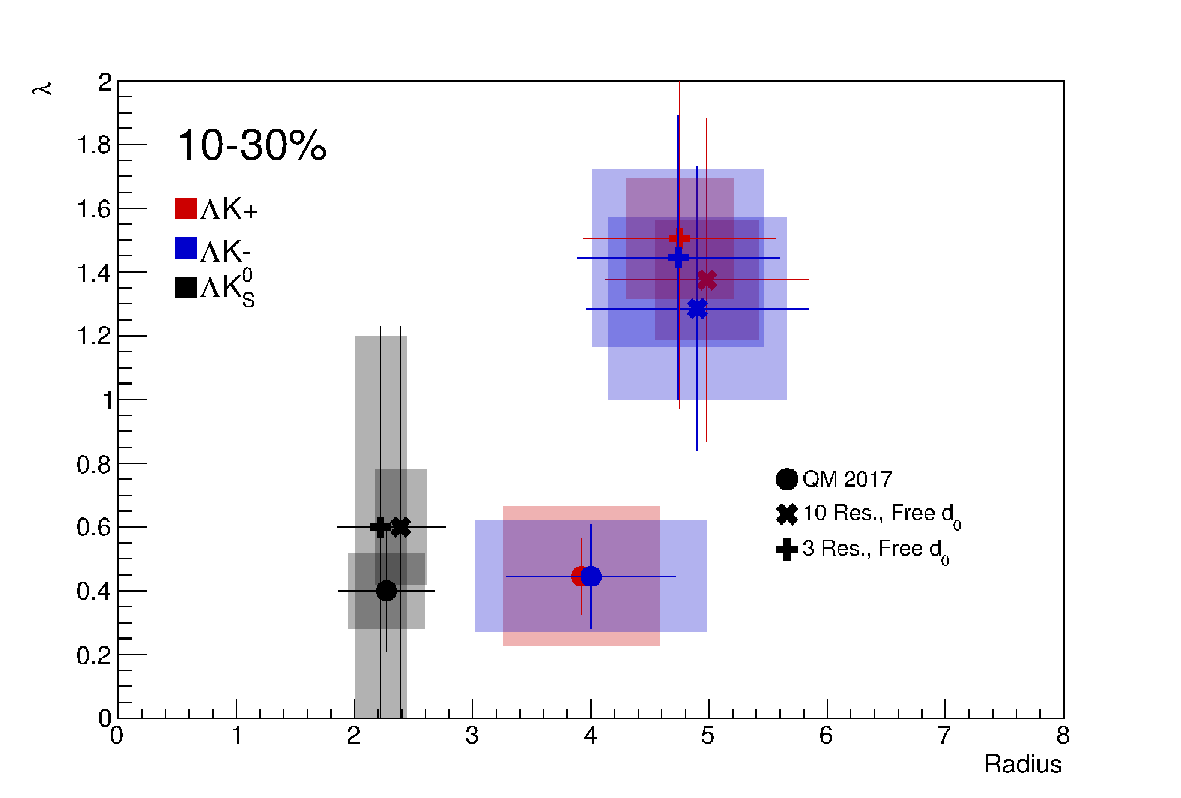
\includegraphics[width=\textwidth]{7_ResultsAndDiscussion/Figures/CompareAllRadiusvsLambdaAcrossAnalyses_1030_10ResAnd3Res_10and3SeparateOnly_FreeD0Only.pdf}
  \caption[$\lambda$ vs. R (10-30\% Centrality)]{Extracted $\lambda$ vs Radius results, for the 10-30\% centrality bin, for all of our $\Lambda$K systems.  The plot shows results including no residuals (circles), 10 residual pairs (X), and 3 residual pairs (+).  Note, $\Lambda$K$^{+}$ on the plot is shorthand for $\Lambda$K$^{+}$ and $\bar{\Lambda}$K$^{-}$, and similar for the others.}
  \label{fig:LambdavsR_1030_FreeD0Only}
\end{figure}

\begin{figure}[h]
  \centering
  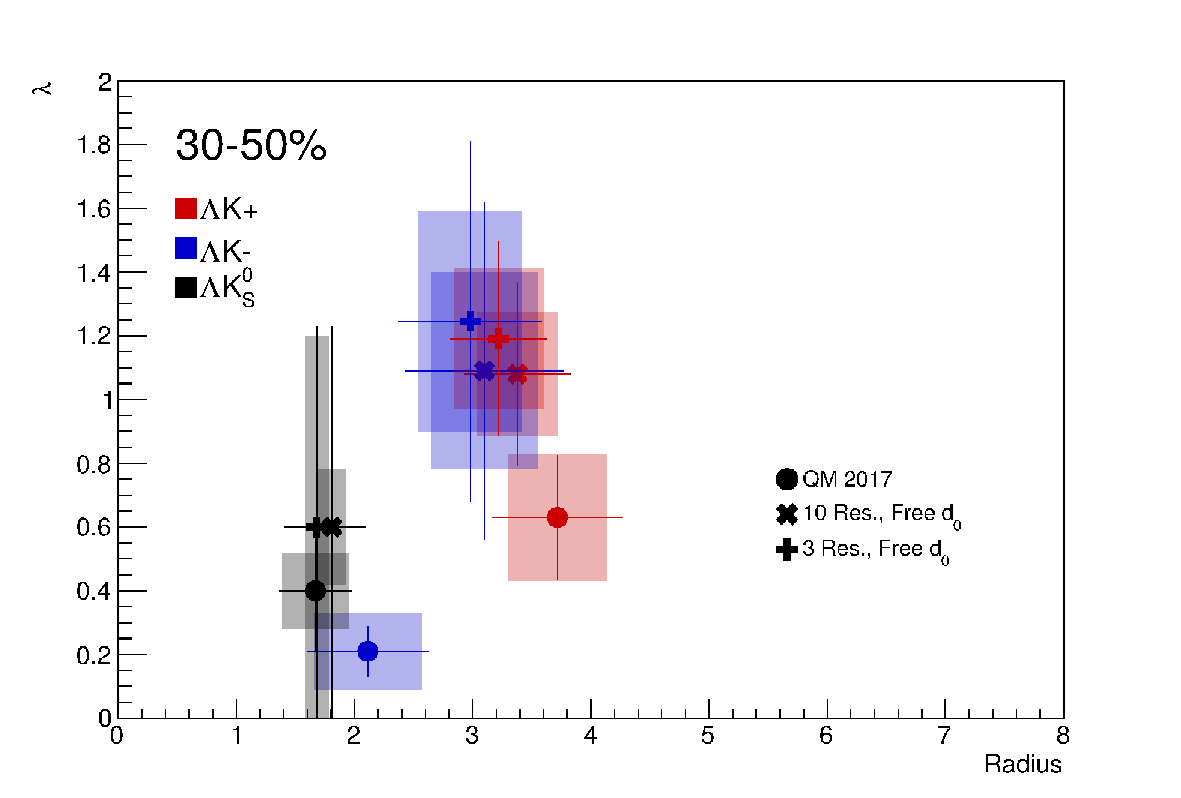
\includegraphics[width=\textwidth]{7_ResultsAndDiscussion/Figures/CompareAllRadiusvsLambdaAcrossAnalyses_3050_10ResAnd3Res_10and3SeparateOnly_FreeD0Only.pdf}
  \caption[$\lambda$ vs. R (30-50\% Centrality)]{Extracted $\lambda$ vs Radius results, for the 30-50\% centrality bin, for all of our $\Lambda$K systems.  The plot shows results including no residuals (circles), 10 residual pairs (X), and 3 residual pairs (+).  Note, $\Lambda$K$^{+}$ on the plot is shorthand for $\Lambda$K$^{+}$ and $\bar{\Lambda}$K$^{-}$, and similar for the others.}
  \label{fig:LambdavsR_3050_FreeD0Only}
\end{figure}

\end{comment}
%%%%%%%%%%%%%%%%%%%%%%%%%%%%%%%%%%%%%%%%%%%%%%%%%%%%%%%%%%%%%%%%%%%%%%%%%%%%%%%%%%%%%%%%%%%%%%%


\begin{figure}[h!]
  \centering
  %%----start of first subfigure---  
  \subfloat[Extracted scattering parameter results, Im(f$_{0}$) vs. Re(f$_{0}$), with d$_{0}$ to the right, for all of our $\Lambda$K systems. ]{
    \label{fig:Results_FreeD0Only:a}
    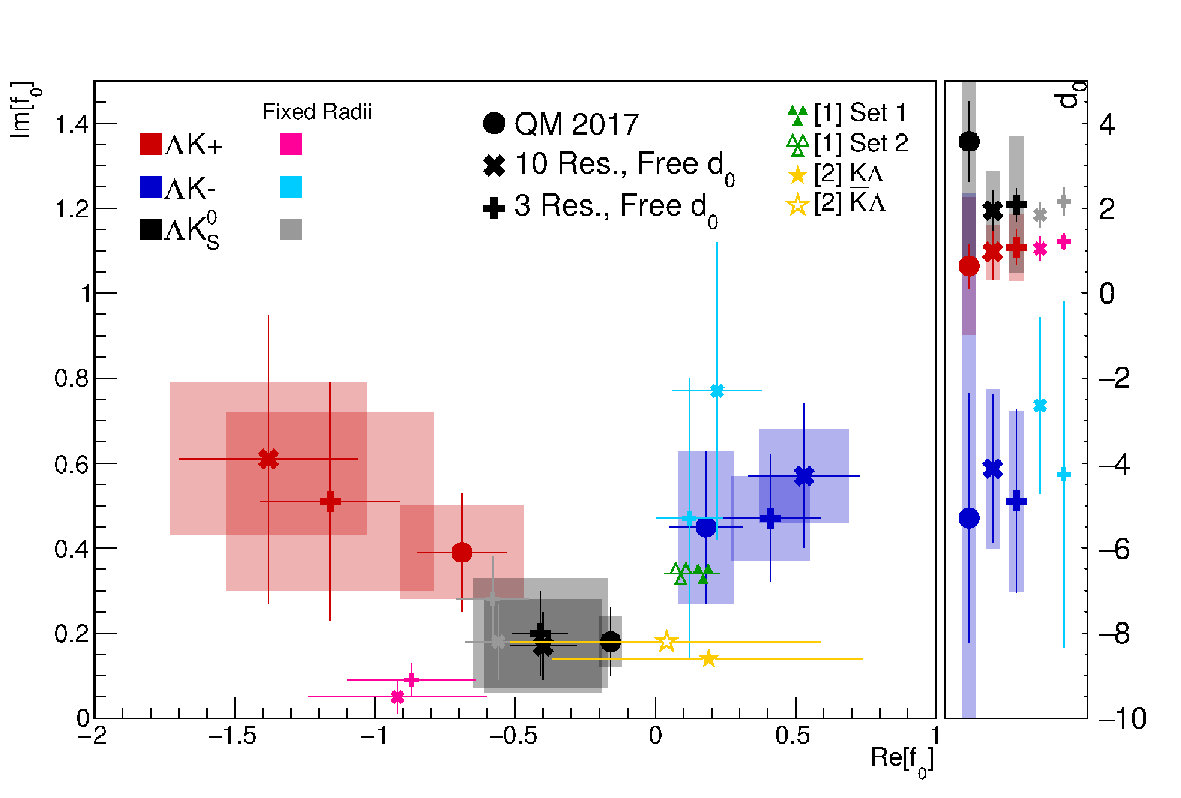
\includegraphics[width=0.49\textwidth]{7_ResultsAndDiscussion/Figures/CompareAllReF0vsImF0AcrossAnalyses_10ResAnd3Res_10and3SeparateOnly_FreeD0Only_wFixedRadiiResults_wScattLenPredictions.pdf}}
  %%----start of second subfigure---
  \subfloat[Extracted $\lambda$ vs Radius results, for the 0-10\% centrality bin, for all of our \LamKchP systems.]{
    \label{fig:Results_FreeD0Only:b}
    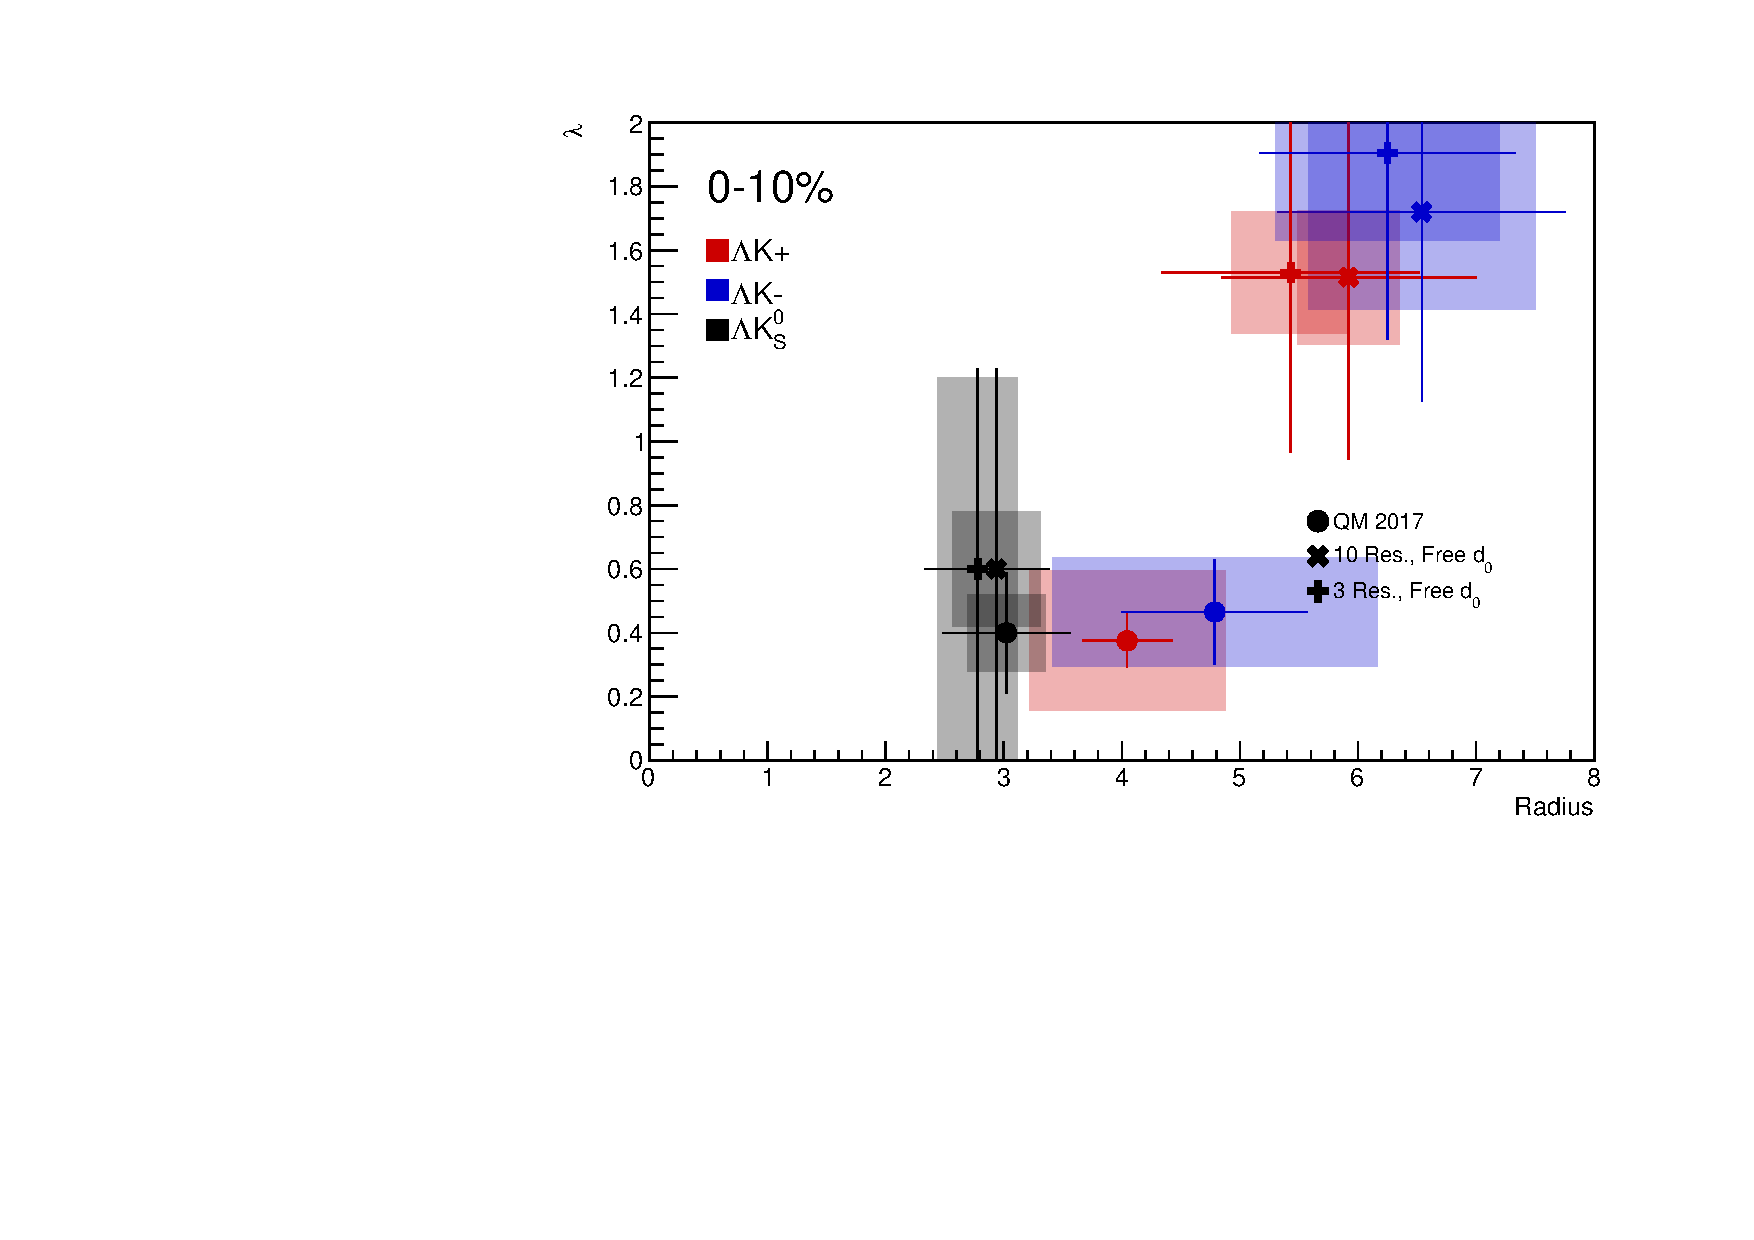
\includegraphics[width=0.49\textwidth]{7_ResultsAndDiscussion/Figures/CompareAllRadiusvsLambdaAcrossAnalyses_0010_10ResAnd3Res_10and3SeparateOnly_FreeD0Only.pdf}}
  \\  
  %%----start of third subfigure---
  \subfloat[Extracted $\lambda$ vs Radius results, for the 10-30\% centrality bin, for all of our \LamKchP systems.]{
    \label{fig:Results_FreeD0Only:c}
    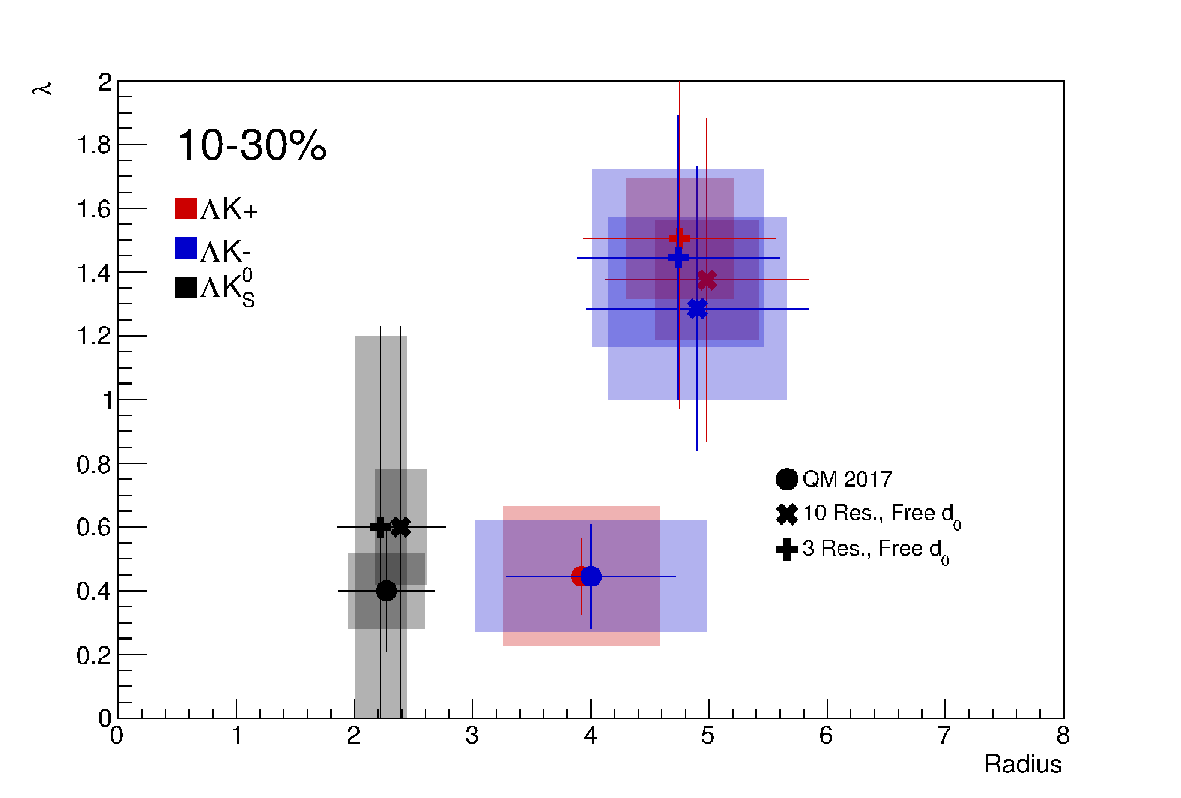
\includegraphics[width=0.49\textwidth]{7_ResultsAndDiscussion/Figures/CompareAllRadiusvsLambdaAcrossAnalyses_1030_10ResAnd3Res_10and3SeparateOnly_FreeD0Only.pdf}}    
  %%----start of fourth subfigure---
  \subfloat[Extracted $\lambda$ vs Radius results, for the 30-50\% centrality bin, for all of our \LamKchP systems.]{
    \label{fig:Results_FreeD0Only:d}
    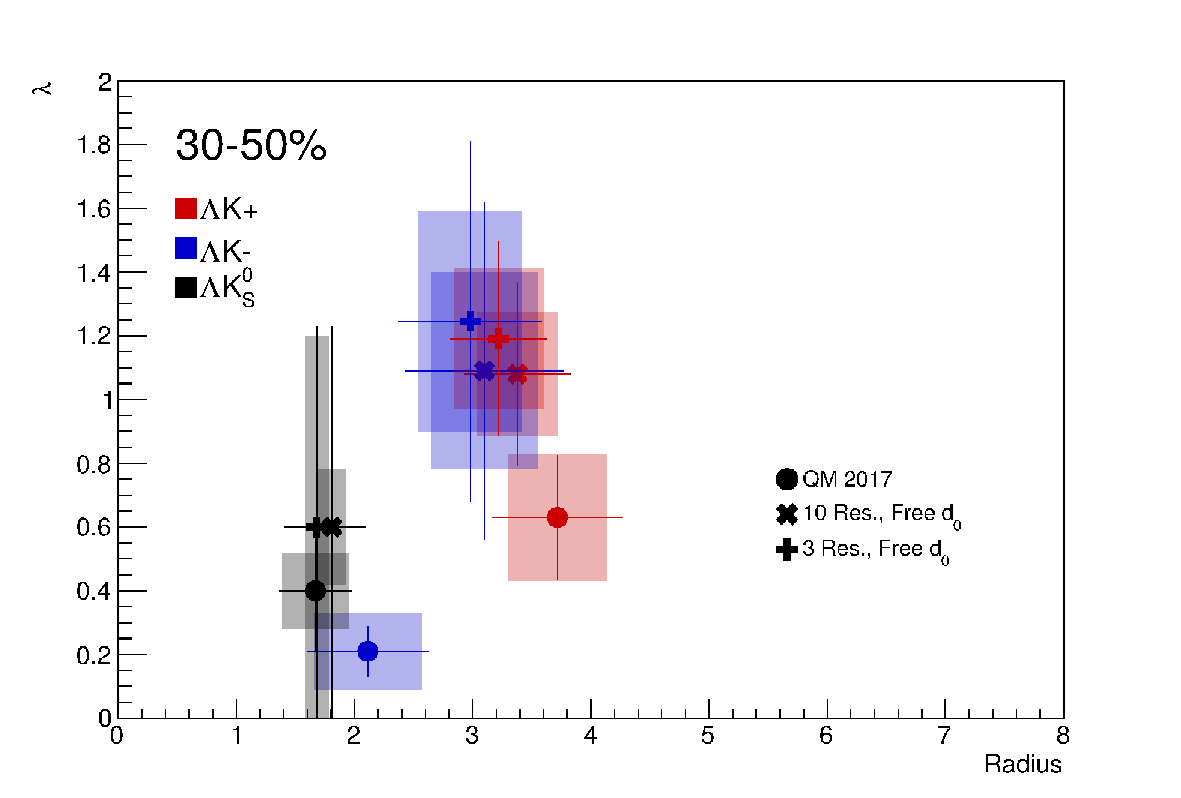
\includegraphics[width=0.49\textwidth]{7_ResultsAndDiscussion/Figures/CompareAllRadiusvsLambdaAcrossAnalyses_3050_10ResAnd3Res_10and3SeparateOnly_FreeD0Only.pdf}}       
  %%----overall caption----
  \caption[Fit Results]{Extracted fit results for all of our $\Lambda$K systems across all studied centrality bins (0-10\%, 10-30\%, 30-50\%).  The plots show results including no residuals (circles), 10 residual pairs (X), and 3 residual pairs (+).  Note, \LamKchP on the plot is shorthand for \LamKchP and \ALamKchM, and similar for the others.  In Fig. \ref{fig:Results_FreeD0Only:a}, the lighter color markers (pink, sky blue, gray) show the extracted parameters when we fix the radii to roughly align with the $m_{\mathrm{T}}$-scaling plot (Fig. \ref{fig:mTScalingOfRadii_NoRes}).  Additionally, the green \cite{Liu:2006xja} and yellow \cite{Mai:2009ce} points show theoretical predictions made using chiral perturbation theory.}
  \label{fig:Results_FreeD0Only}
\end{figure}


\clearpage

\subfile{7_ResultsAndDiscussion/7.1.1_ResultsLamK_NoRes.tex}
\subfile{7_ResultsAndDiscussion/7.1.2_ResultsLamK_3Res.tex}
\subfile{7_ResultsAndDiscussion/7.1.3_ResultsLamK_10Res.tex}
\subfile{7_ResultsAndDiscussion/7.1.4_ResultsLamK_FitMethodComparisons.tex}

\end{document}